\begin{figure}[h]
	\begin{center}
		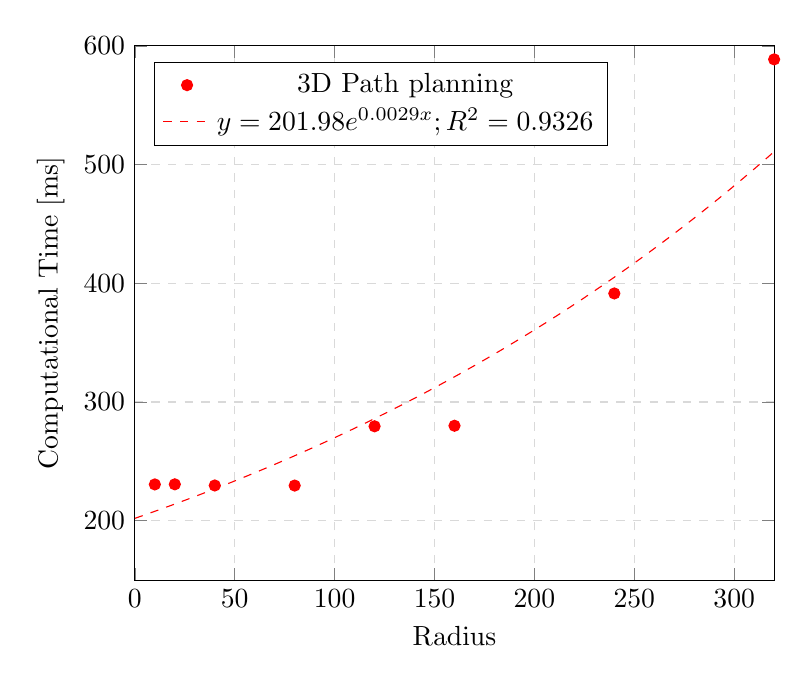
\begin{tikzpicture}
			\begin{axis}[
				width=0.8\linewidth, % Scale the plot to \linewidth
				grid=major, 
				grid style={dashed,gray!30},
				xlabel={Radius}, % Set the labels
				ylabel={Computational Time [ms]},
				legend pos=north west,
				xmin=0,
				xmax=320,
				ymin=150,
				ymax=600,
				]
				
				
				%2d test data
				\addplot[only marks, color=red]
				table[row sep=crcr]{
					10 230.5572793  \\
					20 230.6465518  \\
					40 229.669491   \\
					80 229.5970721  \\
					120 279.5138153 \\
					160 279.9739437 \\
					240 391.4133536 \\
					320 588.5701149 \\
				}; 
				\addlegendentry{3D Path planning}
				
				%2d test regression
				\addplot[domain=0:320, samples=100,no marks, color=red, style=dashed]
				{201.98*e^(0.0029*x)};
				\addlegendentry{$y = 201.98e^{0.0029x}; R^2 =  0.9326$} 
			\end{axis}
		\end{tikzpicture}
		\caption{In this plot the correlation between increased collision detection and computational time, for the three-dimensional path-planning algorithm }
		\label{plot:3dCollisionExp}
	\end{center}
\end{figure}